\section{Mechanisms in Nanofiltration}
\label{ion_afsnit}



%modeling performance of NF membranes:
NF membrane properties lie somewhere between that of non-porous RO membranes where transport is governed by solution-diffusion mechanism, and those of porous UF where size exclusion and charge effects are main factors in separation. 
%NF membranes are often regarded as a collection of capillaries with structural properties (e.g. pore size) and electrical properties, this means separation properties in NF membranes include both size sieving and electrostatic effects. \citep{wangPoreModelNanofiltration2021} 
%Meaning solute transport in NF membranes are affected by multiple mechanisms.
Bowen et al. 1997 used AFM to verify the existence of discrete pores within NF membranes. \citep{bowenCharacterisationNanofiltrationMembranes1997}
%close to the sizes obtained from 'pore models'.
Another study by Schaep et al. 1998 showed that membrane charge density was dependent on salt type and concentration in the feed solution. \citep{schaepInfluenceIonSize1998} 
%The combination of small pore diameters with electrically charged membranes result in a complex mechanism for solute retention. 
Based on this work the 'Donnan Steric Pore Model with Dielectric Exclusion' (DSPM-DE) model was proposed which is the most commonly accepted model used in describing NF and the underlying separation mechanisms. \citep{NanoFiltran_computer_2008} \citep{wangPoreModelNanofiltration2021} 
This model is a mechanistic model representing the membrane as an active layer having a nano-porous structure, and describe solute partitioning at solute-membrane interfaces, see \cref{fig:NF_illustration_transport}.
%where partitioning and ion transport has to be modeled.
%Where the concentration at the membrane ($c_m$) also is affected by CP. 
Exclusion in the DSPM-DE model is described by partitioning i.e. the distribution of ions at the entrance ($c_{i,0}$) and exit ($c_{i,N}$) of membrane pores by three mechanisms: steric, dielectric and Donnan exclusion.
The DSPM-DE model describes the membrane by certain characteristics; pore size, thickness, porosity, charge and pore dielectric constant. 
Transport of solutes inside the pores is described by the extended Nernst-Planck equation (ENP). \citep{wangPoreModelNanofiltration2021}
%To accurately calculate the concentration profile across the membrane, discretization can be used. 
Where the active membrane layer is divided into $n$ sub-sections of non-overlapping control volumes, %the concentration and electric potential is calculated, 
and the ENP is applied in each section, ($c_{i,n}$) see \cref{fig:NF_illustration_transport}. 
\citep{NanoFiltran_computer_2008} \citep{MIT_2018_DSPM_DE_Fabrication} 
%"For sufficiently refined grids, a linear variation of the dependent variables can accurately represent the exact variation between two consecutive grid nodes and therefore the central differences scheme is adequate for the discretization of the ENP equations [52]." kilde = NanoFiltran artikel 2008.
This makes the DSPM-DE model able to describe the concentration in the permeate stream, based on feed concentration and membrane characteristics. \citep{wangPoreModelNanofiltration2021}
%\textcolor{blue}{Slut af med noget om at det kræver mange steps og iterationer at modelere NF correct.}
%The overall transport is then modeled by evaluating partitioning at the feed side, transport  through the membrane by ENP and partitioning at the permeate side.



\begin{figure}[H]
    \centering
    \begin{tikzpicture}
\coordinate (A) at (13,0);
\coordinate (B) at (2,2);
\coordinate (C) at (3.5,3.5);
\coordinate (NF1) at (3.5,5);
\coordinate (NF2) at (4,4.35);
\coordinate (NF3) at (6,3.55);
\coordinate (NF4) at (8.5,3.5);
\draw  (0,0) node[below]{$x$} --(A);

\draw (0,2)node[above]{$c_f$}--(B);
\draw (B) to[out=0,in=265] (C) node[left]{$c_m$};
\draw (C)++(0,1.5)node[left]{$c_{i,0}$} to[out=300,in=180] (NF4) node[right]{$c_{i,N}$};
\draw (8.5,1)--node[above]{$c_p$}++(2,0);

\draw[dashed] (B)--+(0,5)--+(0,-2) node[below]{$\delta$};

\draw[pattern = dots] (C)++(0,-3.5) rectangle +(5,7);
\fill[blue,opacity=0.3] (C)++(0,-3.5) rectangle +(5,7);
\filldraw[black!70] (NF1) circle (0.1cm);
\filldraw[black!70] (NF2) circle (0.1cm);
\filldraw[black!70] (NF3) circle (0.1cm);
\filldraw[black!70] (NF4) circle (0.1cm);
% \draw[   decoration={markings,
%         mark=at position 1 with {\arrow[scale=2.5,>=latex]{>}}
%         },
%     postaction={decorate}] (5.5,4)--node[above]{$J\cdot c$}++(1.5,0);
% \draw[   decoration={markings,
%         mark=at position 1 with {\arrow[scale=2.5,>=latex]{>}}
%         },
%     postaction={decorate}] (7.5,1)--node[above]{$D\cdot \frac{dc}{dx}$}++(-1.5,0);

% \draw[   decoration={markings,
%         mark=at position 1 with {\arrow[scale=2.5,>=latex]{>}}
%         },
%     postaction={decorate}] (9.5,4)--node[above]{$J\cdot c_p$}++(1.5,0);

\node at (1,6) {Bulk Feed};
\node at (2.8,6) {CP};
\node[draw, fill=white] at (6,6) {Membrane Active Layer};
\node at (9.5,6) {Permeate};
\node[above right=2pt,draw, fill=white] at (NF2) {$c_{i,1}$};
\node[above right=2pt,draw, fill=white] at (NF3) {$c_{i,n}$};
%\node at (6.6,6.2) {Boundary};
%\node at (6.6,5.8) {Layer};

%\draw [decorate,
%     decoration = {calligraphic brace}] (3,-1)--(2,-1);
    
\draw [decorate,
    decoration = {brace,amplitude=5pt}] (4,-0.1)--++(-1,0);
\node at (3.5,-0.6) {$\phi_S\phi_{Don}\phi_{DE}$};
\draw [decorate,
    decoration = {brace,amplitude=5pt}] (9,-0.1)--++(-1,0);
\node at (8.5,-0.6) {$\phi_S\phi_{Don}\phi_{DE}$};


\draw[white,fill=white] (4,0.74) rectangle +(3.5,0.52);
\node at (6,1) {ENP};
\draw  (4,1.26)  -- +(3.5,0);
\draw  (4,0.74)  -- +(3.5,0);
\fill[white] (7.5,0.74) --(7.5,1.26)--(8,0.99)--cycle; 
\draw  (7.33,0.64)  -- (8,1);
\draw  (7.33,1.36)  -- (8,1);
\end{tikzpicture}
    \caption{Transport over membrane illustration for a ion with opposite charge of the membrane. }
    \label{fig:NF_illustration_transport}
\end{figure}

%"Modeling transport of species across NF memrbane has to consider, solute transport within the active layer, concentration polarization, and solute partitioning at Electrochemical equilibrium" %https://dspace.mit.edu/bitstream/handle/1721.1/114293/LABBAN_preprint-Relating_Transport_Modeling_to_NF_Membrane_Fab.pdf;jsessionid=600BFB9171808D243A9B10A698E7608E?sequence=1. 

\subsection{Interface Partitioning Mechanisms}
Despite the DSPM-DE model being used frequently it has limitations as it must be applied based on multiple assumptions.  
Firstly transport through the support layer is ignored, due to its much larger pore size compared to the active layer. 
The active layer is assumed to have uniform cylindrical pores, where water flux is modeled by Hagen-Poiseuille equation and a concentration gradient across the length of the membrane is also ignored. 
%Electro-neutrality is assumed to be maintained, both at solution-membrane interface and within the pores. 
Lastly the NF process must be in steady state.  \citep{wangPoreModelNanofiltration2021}

%There is generally agreement that partitioning at NF membranes is governed by a combination of steric hindrance, Donnan potential and Dielectric exclusion (DE).

\textbf{Size exclusion}\\
%\prettyinpink{man kan lave en lille figur til dette, men det er nok ikke nødvendigt}
%Fra Nanofiltration principles applications and new materials:
%Size exclusion is because big ball no go through small hole
Steric hindrance is based on the physical or sieving exclusion of solute ions from the pore walls of the membrane and can be described by the partition coefficient.
Solutes are typically modelled as spheres with stokes radius determining their size.
For the interface partitioning into an NF membrane diffusion dominates the transport of ions, which means that solutes larger than the pore size are always excluded but those of a size smaller than the pore size do not always enter the pore, and are excluded with a certain size-dependant probability. \citep{wangPoreModelNanofiltration2021}
The probability of entering a pore for an ion \textit{i} is the steric exclusion factor $\phi_{S,i}$.  
\begin{align}
\phi_{S,i} = \left(1-\frac{r_i}{r_p}\right)^2, \text{ for  $r_i < r_p$}
\end{align}
where $r_i$ is the Stokes radius of the solute and $r_p$ is the radius of the membrane-pore.
The conclusions of this are that smaller ions pass more easily and smaller pores have greater hindrances. 
This coefficient, describing geometric exclusion of the center of ions by the pore, is also the average concentration inside the pore divided by the concentration outside. \citep{nanofiltration_2021_bog_fraMorten}
Charge density of the ion also plays a role in size-exclusion of it, as ions with a greater charge density have smaller hydrated radii and greater hydration energy.
The degree to which ions are capable of losing their hydration shell affects their exclusion which is not included in the DSPM-DE model.  \citep{wangPoreModelNanofiltration2021}
% \begin{figure}[H]
%     \centering
%     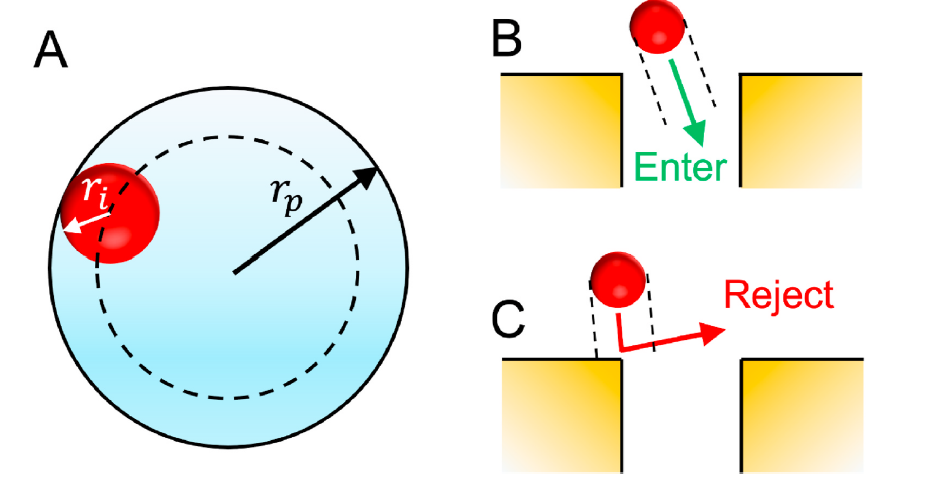
\includegraphics[width=0.7\textwidth]{Billeder/teori/size_exclusion.png}
%     \caption{Size exclusion illustration}
%     \label{fig:size_exclusion}
% \end{figure}

\begin{figure}[H]
    \centering
    \begin{tikzpicture}[scale=0.8]
\coordinate (A) at (13,0);
\coordinate (B) at (2,2);
\coordinate (C) at (3.5,3.5);

\def \x {3.5cm};
\def \y {1cm};
%\draw[line width=2pt,fill=blue!20] (0,0) circle (\x);
\draw[shading = axis,rectangle, left color=blue!40, right color=white,shading angle=135,line width=2pt,fill=blue!20] (0,0) circle (\x);
\shade[ball color=black!50] (canvas polar cs:angle=160,radius=\x-\y) circle (\y);
%\draw[fill=black!40] (canvas polar cs:angle=160,radius=\x-\y) circle (\y);
\draw[line width=2pt,dashed] (0,0) circle (\x-\y);

\draw[line width=2pt] [-{Latex[scale=1]}](0,0)  -- node[anchor=south] {\huge $r_p$}(canvas polar cs:angle=40,radius=\x);
\draw[line width=1.5pt] [-{Latex[scale=1]}](canvas polar cs:angle=160,radius=\x-\y)node[anchor=west] {\huge\textcolor{white}{$r_i$}}  -- (canvas polar cs:angle=160,radius=\x);
%


\end{tikzpicture}
    \caption{Size exclusion illustration}
    \label{fig:size_exclusion}
\end{figure}

\textbf{Dielectric exclusion}\\
%What is dielectric constant: factor of how much electric field between two charges is decreased compared to vacuum. 
Dielectric exclusion (DE) arises from differences in how charged solutes interact with point charges inside and outside the membrane pores.
The dielectric constant of a given solvent can be smaller in narrow pore such as the pores of an NF membrane. 
This lower dielectric constant within the pores results in a solvation energy barrier for ions that hinders transportation of ions to regions with lower dielectric constants, as it is energetically favorable for the hydrated ions to stay in the bulk solution which has a comparatively higher dielectric constant. 
The dielectric exclusion factor for ions $\phi_{DE,i}$ is based on the Born model and is a function of change in solvation energy between the two environments $\Delta  W_i$ , 

\begin{ceqn}
    \begin{align}
   \phi_{DE,i}=exp\left(-\frac{-\Delta W_i}{k_B \cdot T}\right)
    \end{align} 
 \end{ceqn}
%$k_B$ is the Boltzmann constant. 
The change in solvation energy ($\Delta W$) is a result of the differences in dielectric constant between bulk solution and in the nano-pores: 

\begin{ceqn}
    \begin{align}
   \Delta W_i = \frac{z_i^2e^2}{8\pi\varepsilon_0 r_i}\cdot \left(\frac{1}{\varepsilon_b}-\frac{1}{\varepsilon_p}\right)
    \end{align} 
 \end{ceqn}

$\epsilon_0$, $\epsilon_b$ and $\epsilon_p$ are the dielectric constants in vacuum, in the bulk solvent, and in the nano-pore, respectively.
$z_i$  is the valence of the ion $i$ and $e$ the elemental charge.
The lower dielectric exclusion in the pore can be described by the favorable orientation of water molecules near the pore wall, see \Cref{fig:dielectric_exclusion}, which results in a area with a lower dielectric constant than bulk $\varepsilon^*$.
The overall dielectric properties of the membrane pore can then be described by an area average of those differing constants:

\begin{ceqn}
    \begin{align}
        \varepsilon_p = \varepsilon^* +(\varepsilon_b - \varepsilon^*) \left(1-\frac{\delta}{r_p}\right)^2
    \end{align}
\end{ceqn}

Dielectric exclusion is applied to charged ions, but it might also be applicable to neutral hydrated molecules, which is not included in the Born model of DE.
In the same manner dielectric exclusion is only associated with solvation, but dehydration is not considered in this model although it is theorized to affect the partitioning of solutes. \citep{wangPoreModelNanofiltration2021} 

\begin{figure}[H]
    \centering
    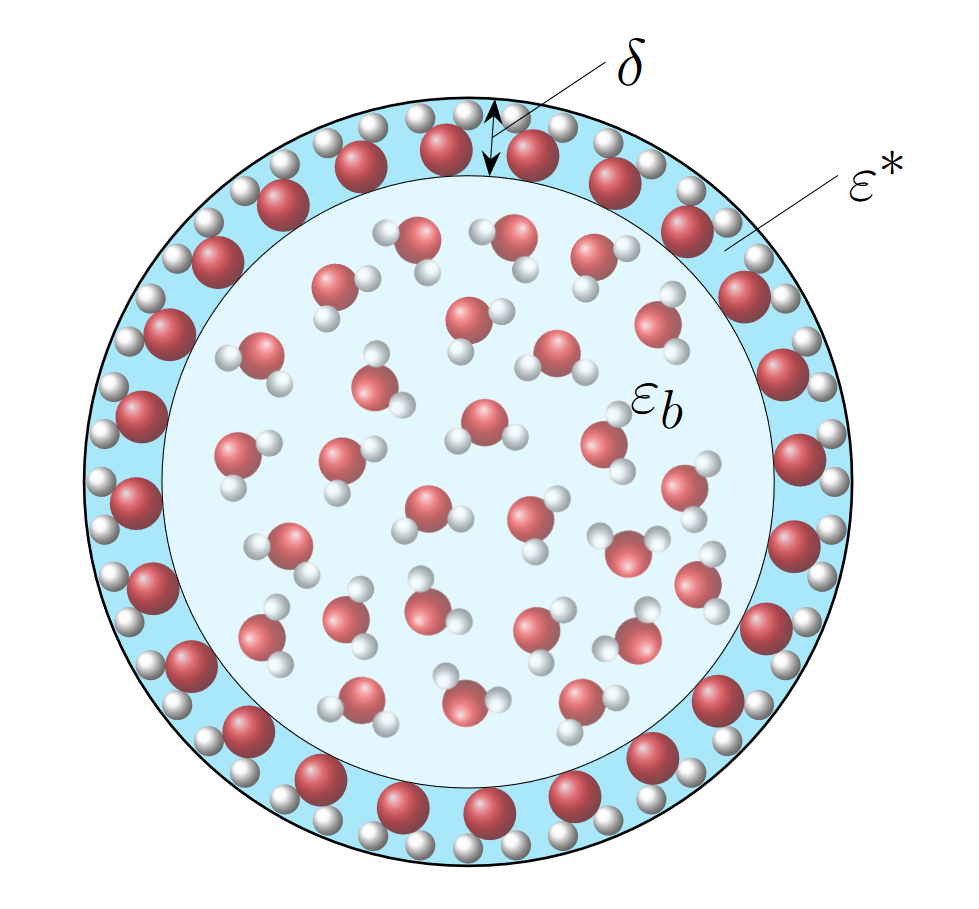
\includegraphics[width=0.6\textwidth]{Billeder/teori/Dielectric_exclusion.png}
    \caption{Ilustration of dielectric exclusion}
    \label{fig:dielectric_exclusion}
\end{figure}


\textbf{Donnan exclusion}\\
The Donnan effect describes the interaction of small diffusible ions on either side of a charged semipermeable membrane. \rod{(kilde OS ChangRaymond)}
NF membranes typically contain fixed charges due to dissociation of surface groups. 
Solute ions with the same charge sign as the membrane surface are called co-ions (e.g. \ce{Cl-} or \ce{SO4}  are co-ions of a negatively charged membrane) and those of the opposite charge are named counter-ions.
Due to the differences in ion concentrations between feed bulk and membrane matrix plus membrane matrix and permeate there exists Donnan potentials over those interfaces on both sides of the membrane. \citep{wangPoreModelNanofiltration2021}
The exclusion factor $\phi_{D,i}$, which is the partitioning equilibrium of the ion \textit{i} at those interfaces,  expressed as: \citep{wangPoreModelNanofiltration2021}

% Donnan potentials exist at the membrane - solution interfaces on both sides of the membrane due to the differences on ion concentration between solution and membrane matrix.


% \begin{ceqn}
%     \begin{align}
%   \frac{C_{II}}{C_I}=exp\left(-\frac{z_i F}{R \cdot T}\cdot \psi_{Don}\right)
%     \end{align} 
%  \end{ceqn}

\begin{ceqn}
    \begin{align}
   \phi_{D,i}=exp\left(-\frac{z_i e}{k_B \cdot T}\cdot \Delta\psi_D\right)
    \end{align} 
 \end{ceqn}

Where $\psi_{Don}$ is the Donnan potential over the membrane, being the potential difference between just inside the membrane matrix and in solution. 
For co-ionic solutes, Donnan exclusion reduces the ion partition coefficient (interface between feed bulk and pore opening) making membranes exhibit higher rejection than for similarly sized uncharged solutes.
The opposite is true for counter-ionic solutes, where Donnan exclusion enhances their concentration in the membrane matrix, increasing the transmission/passage of the ion. \citep{nanofiltration_2021_bog_fraMorten}
This is opposite to dielectric exclusion which affects both co-ions and counter-ions. \citep{wangPoreModelNanofiltration2021}
%opposite to Donnan exclusion where only co-ions are excluded.%non-steric....
Furthermore charge neutrality conditions are also enforced between these solution/membrane matrix interfaces according to equilibria: \citep{wangPoreModelNanofiltration2021}

\begin{ceqn} 
    \begin{align}
     \sum_{i=1}^{N} z_ic_{i,f}  = 0 
              \label{eq:neutrality_feed}
    \end{align} 
\end{ceqn}  

\begin{ceqn} 
    \begin{align}
     \sum_{i=1}^{N} z_ic_{i,p}  = 0 
              \label{eq:neutrality_permeate}
    \end{align} 
\end{ceqn}  

%Where $c_{i,f}$ and $c_{i,p}$ is the concentration in feed bulk and permeate respectively, CP should also be considered. \citep{wangPoreModelNanofiltration2021}

\begin{figure}
    \centering
    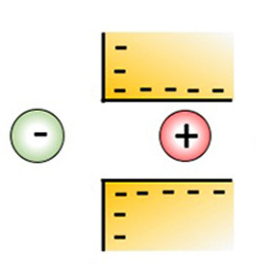
\includegraphics[width=0.4\textwidth]{Billeder/teori/donnan_exclusion.png}
    \caption{Illustration Donnan exclusion, clearly}
    \label{fig:donnan_exclusion}
\end{figure}
%NF bogen:
%"The charges give rise to electrical double layers next to the wall surface"
% "Transmission coefficients larger than unity may mean preferential (relative to
% the solvent) transfer of the solute and negative rejections. (At high volume flows,
% transmission coefficients larger than 1 imply negative rejection, as the rejection
% approaches the reflection coefficient, which is defined as one minus transmission
% coefficient.) However, in zero-current pressure-driven membrane processes,
% the electromigration counter flow generated by spontaneously arising electric
% fields largely compensates (sometimes even overcompensates) the enhanced partitioning
% of counter-ions. Nonetheless, with salts whose counter-ions have lower
% mobility than co-ions, the purely Donnan exclusion mechanism can give rise
% to slightly negative rejections at small to moderate dimensionless fixed-charge
% concentrations"




%Investigating transport properties of nanofiltration membranes by means of a steric, electric and dielectric exclusion model


% The most accepted model used to describe transport phenomena in NF are the Extended Nernst–Planck differential equations for each ion coupled with two electroneutrality conditions for the ion fluxes and local concentrations.
% These contain coefficients which must be determined by thermodynamic and kinetic models for ion exclusion. 

% These may instead be determined by the models based on hindered transport: steric dielectric and donnan SDE.

% A different approach is the solution diffuion model which assumes ion transport based on a solution diffusion mechanism. This has shown to give good results for ionic species in RO and may be applicaple to NF membranes especially improving the prediction of the high sulfate/chloride selectivity in comparison with the nano-porous approach.
% "In the case of electrolyte mixtures, coupling between the trans-membrane fluxes of different ions via the electric field of membrane potential has to be explicitly taken into account."
% "called solution-diffusion-film model (SDFM), which assumes that solute transport occurs via diffusion and electric migration through both the membrane and the concentration-polarization layer where it also occurs via convection."


\textbf{Complete Exclusion Scheme}\\
The total partitioning taking into account all three contributions at the feed/membrane interface can be expressed as an equilibrium between the concentration at the membrane wall (i.e. the feed concentration when accounting for CP) and inside the membrane pore. \citep{wangPoreModelNanofiltration2021}
All three mechanisms are multiplied under the assumption that there is no inter-dependence or interaction between the mechanisms.
\begin{ceqn}
\begin{align}
    \frac{\gamma_{i(x=0)}c_{i(x=0)}}{\gamma_{i,m}c_{i,m}}=\phi_S\phi_{D}\phi_{DE}
\end{align}
\end{ceqn}

Where $\gamma_{i(x=0)}$ and $c_{i(x=0)}$ are the activity coefficients and concentration of ion $i$ just inside the membrane, respectively.
The same partitioning can be constructed for membrane/permeate interface at the exit of the pores, where $x=N$ and thus $\gamma_{i(x=N)}$ and $c_{i(x=N)}$ are values for ion $i$ immediately before the permeate stream.
% \begin{ceqn}
% \begin{align}
%     \frac{\gamma_{i(x=N)}c_{i(x=N)}}{\gamma_{i,p}c_{i,p}}=\phi_S\phi_{Don}\phi_{DE}
% \end{align}
% \end{ceqn}
The partitioning is not independent on the transport of the ion inside the membrane as the concentration on ions affect the charge density and potential gradient.
The transport along the pores is also important and is described by the Extended Nerst-Planck equation. \citep{wangPoreModelNanofiltration2021}


\begin{figure}
    \centering
    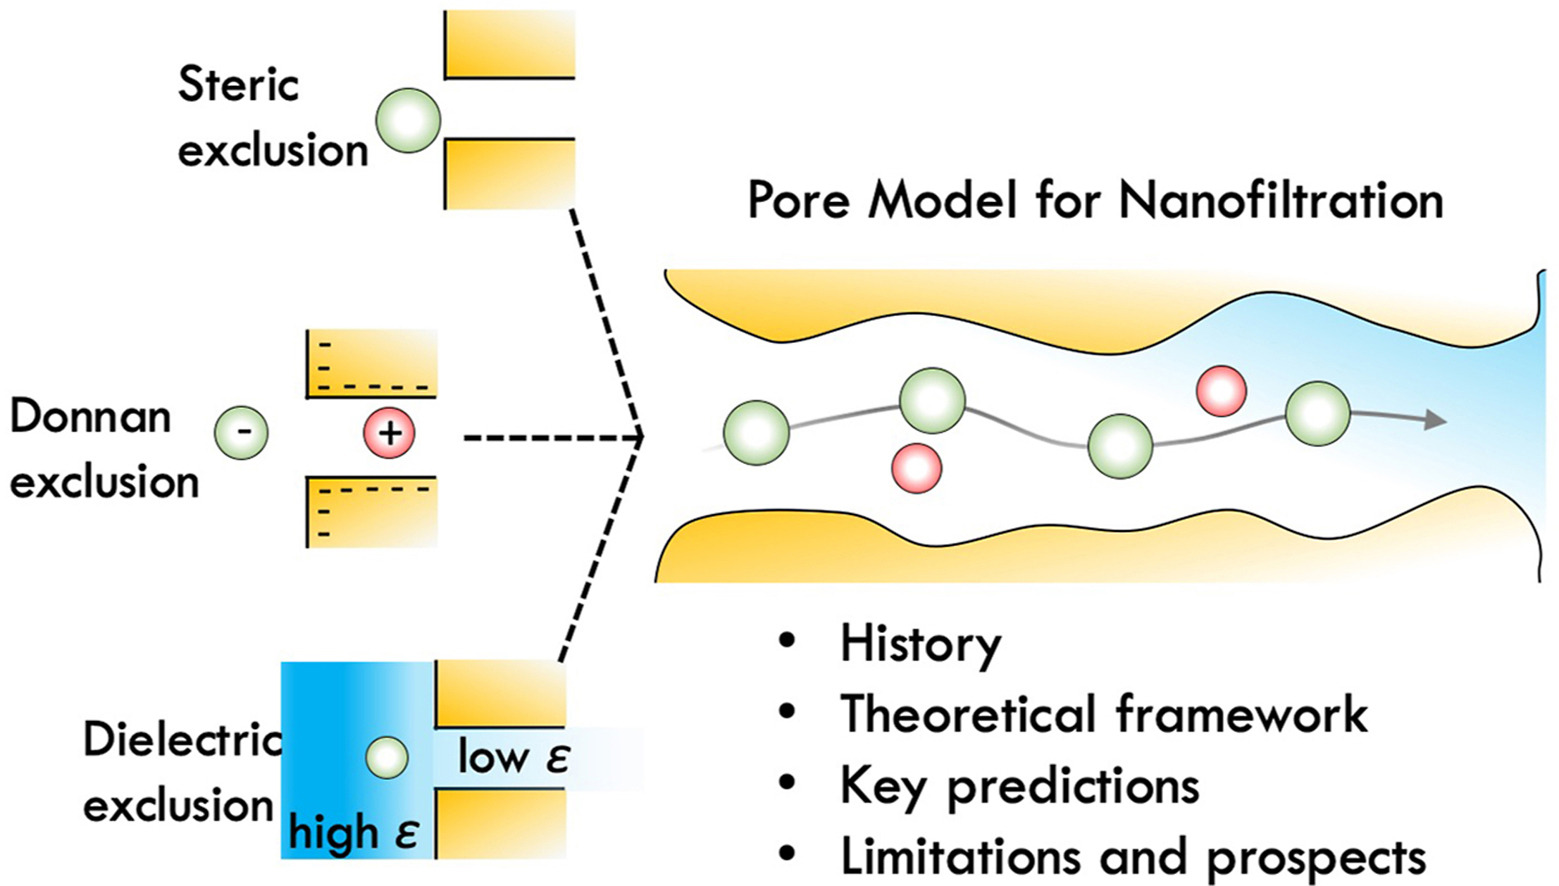
\includegraphics[width=0.7\textwidth]{Billeder/teori/samlet_exclusion.jpg}
    \caption{Illustration of complete rejection scheme}
    \label{fig:complete_exclusion_scheme}
\end{figure}




\subsection{Extended Nerst-Planck Equation }
%The solute transport within the active layer, along membrane pores can be described by the extended Nerst-Planck  equation (ENP), see \cref{eq:Extended_nerst_planck_equation_ENP}.  \citep{MIT_2018_DSPM_DE_Fabrication}
The Extended Nerst-Planck equation consists of three terms describing different driving forces. 
The first term represents diffusive flux of solutes due to a concentration gradient, the second term describes convective flux due to solute flow and the third term is electromigration caused by potential gradient. 
 \citep{wangPoreModelNanofiltration2021}


\begin{ceqn} 
    \begin{align} 
        J_i=-K_{i,d}D_{i,\infty}\frac{dc_i}{dx}+K_{i,c}c_iJ_v-\frac{z_i c_iK_{i,D}D_{i,\infty}F}{RT}\frac{d\phi(x)}{dx}
        \label{eq:Extended_nerst_planck_equation_ENP}
    \end{align}
\end{ceqn}    

Where $J_i$ is the flux of solute \textit{i}, $c_i$ is its concentration and $z_i$ its valency.
$D_{i,\infty}$ is the diffusion coefficient of solute \textit{i} in the bulk solution. 
%$F$ is the Faraday constant, $R$ is the gas constant and $T$ is temperature. 
$J_v$ is volumetric permeate flux and $\phi(x)$ is the electric potential at position $x$ within the pore. 
  \citep{wangPoreModelNanofiltration2021} \citep{MIT_2018_DSPM_DE_Fabrication}
%Electric potential describes the charge of various ions present, and differences in electrical potential can cause ions to either be retained or migrate across the membrane.  
The solute mobility is hindered when the solute size is close to the pore size. \citep{MIT_2018_DSPM_DE_Fabrication} 
Empirical correlations have been proposed to estimate these hindrance factors $K_{i,d}$ and $K_{i,c}$ for diffusion and convection respectively, both are functions of $\lambda_i$ which is $r_i/r_p$.  
%the ratio between solute size and pores size, 
\citep{wangPoreModelNanofiltration2021}

{\small
\begin{ceqn} 
    \begin{align}
       K_{i,d}= \frac{1+\frac{9}{8}ln\lambda_i-1.56\lambda_i+053\lambda_i^2+1.95\lambda_i^3-2.82\lambda_i^4+0.27\lambda_i^5+1.10\lambda_i^6-0.44\lambda_i^7}{(1-\lambda_i)^2},\lambda_i \leq 0.95 \nonumber \\
       K_{i,d}= 0.984 (\frac{1-\lambda_i}{\lambda_i})^{\frac{5}{2}},\lambda_i > 0.95
              \label{eq:Diffusion_hindrance_factor}
    \end{align} 
\end{ceqn}  


}%
\begin{ceqn} 
    \begin{align}
       K_{i,c}= \frac{1+3.867\lambda_i-1.907\lambda_i^2-0.834\lambda_i^3}{1+1.867\lambda_i-0.741\lambda_i^2}
              \label{eq:Convection_hindrance_factor}
    \end{align} 
\end{ceqn}  


%As the dimension of pores approach dimension of solutes, the solute mobility is constricted and diffusion and convection is hindered. 
The validity of applying these hindrance factors to charged solutes has been questioned, as they have been obtained by fitting transport of a neutral solute in a neutral membrane. \citep{wangPoreModelNanofiltration2021} 
Summarised, the ENP equation \ref{eq:Extended_nerst_planck_equation_ENP} indicates that transportation of solutes occurs due to porosity of NF membranes, or due to gradient in concentration of electrical potential. \citep{MIT_2018_DSPM_DE_Fabrication}
In addition %to the ENP \cref{eq:Extended_nerst_planck_equation_ENP} 
electroneutrality condition should also be satisfied within the pore, described by \cref{eq:neutrality_pore}. \citep{MIT_2018_DSPM_DE_Fabrication} \citep{wangPoreModelNanofiltration2021} 

\begin{ceqn} 
    \begin{align}
     \sum_{i=1}^{N} z_ic_i(x) + X(x) = 0 
              \label{eq:neutrality_pore}
    \end{align} 
\end{ceqn}  

Where $z$ and $c$ is valence and concentration at position $x$ within the pore. The charge density $X(x)$ is likewise linked to position $x$ within the pore, this can also be simplified to be homogeneous throughout the membrane and then is reduced to $X$. \citep{wangPoreModelNanofiltration2021}



% \subsection{Rambling thoughts on ions}
% \prettyinpink{Måske nogle konklusioner/overvejelser oven på DSPM så det bliver realteret til vores system?}

% The rejection of an ion is inversely proportional to the diffusivity of the ion.

% The rejection order of ions can be dependant on concentration: at 10 mM R(Na)>R(K)>R(Mg)>R(Ca)
% but at 100 mM R(Mg)>R(Ca)>R(Na)>R(K)
% At low c the electrostatic effect is the major factor responsible for the rejection and at high c the steric hindrance is the governing factor.
%The charge of the membrane also affects the rejection of the species as the ions adsorb to the membrane (donnan exclusion)
%^ fra Separation performance of a nanofiltration membrane influenced by species and concentration of ions


%Rejection in NF systems are mainly steric(size) and donnan(charge) exclusion.







